
\begin{frame}{Phase Diagram of EDT and the Continuum limit}
 \begin{figure}
  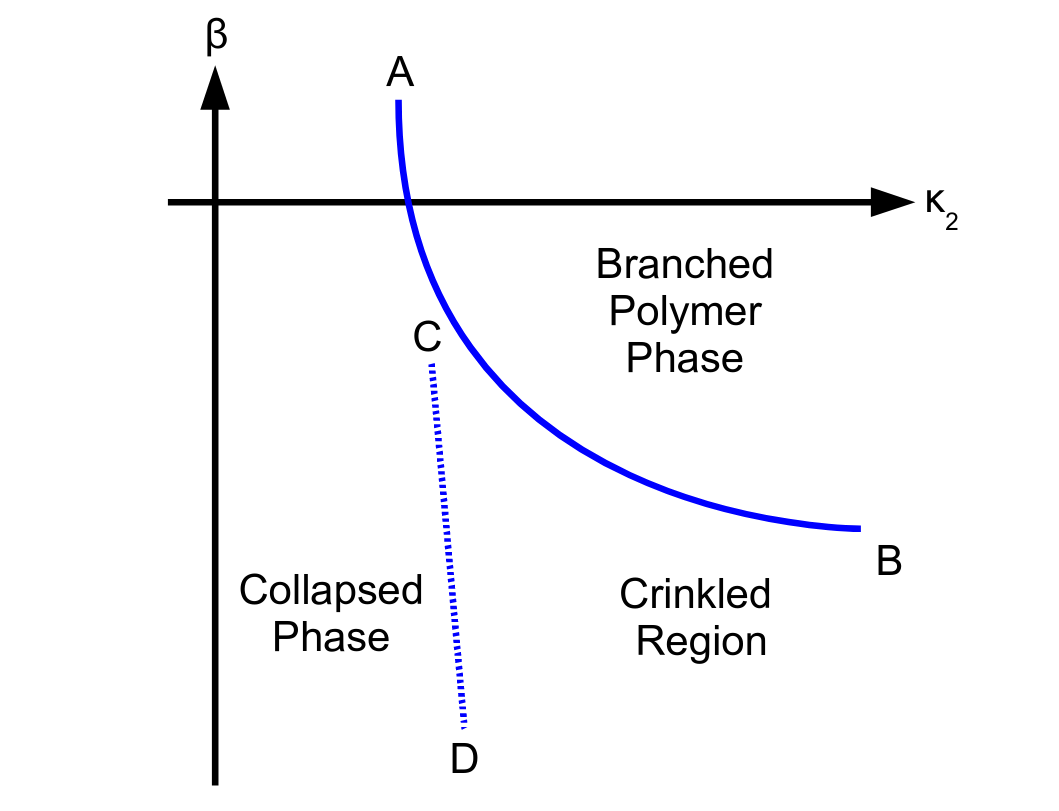
\includegraphics[width=0.6\textwidth]{pics/phase-diagram}
  \caption{SOURCE}
 \end{figure}
\end{frame}

\begin{frame}{Fractal Dimension of the triangulation}
 \begin{columns}
  \begin{column}{0.38\textwidth}
   \begin{figure}
    \centering
    \begin{subfigure}{0.32\textwidth}
     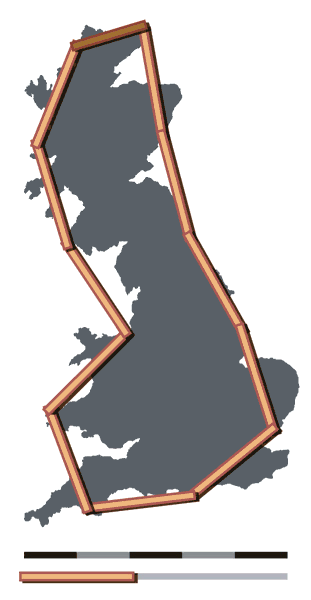
\includegraphics[width=\textwidth]{pics/Britain-fractal-coastline-200km}
     \caption{$\varepsilon=\SI{200}{km}$}
    \end{subfigure}
    \begin{subfigure}{0.32\textwidth}
     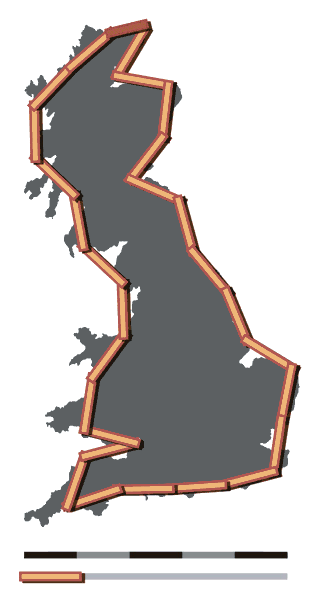
\includegraphics[width=\textwidth]{pics/Britain-fractal-coastline-100km}
     \caption{$\varepsilon=\SI{100}{km}$}
    \end{subfigure}
    \begin{subfigure}{0.32\textwidth}
     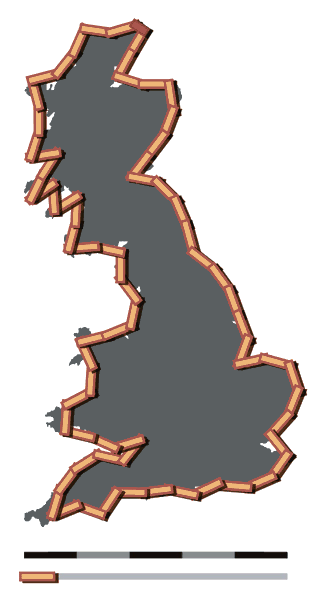
\includegraphics[width=\textwidth]{pics/Britain-fractal-coastline-50km}
     \caption{$\varepsilon=\SI{50}{km}$}
    \end{subfigure}
    \caption{\tiny{Source: \url{https://commons.wikimedia.org/wiki/File:Britain-fractal-coastline-combined.jpg}}}
   \end{figure}
   % Germany: 1.111
   % United Kingdom: 1.215
   % Norway: 1.372
  \end{column}
  \begin{column}{0.58\textwidth}
   \begin{block}{Fractal Dimensions}
    \vspace{0pt}
    \begin{itemize}
     \item Quantifies ''roughness'' of surface
     \item Expect $d=4$ in continuum limit
    \end{itemize}
    \textbf{Box-Counting Dimension}
    \begin{align*}
     d_{\textrm{box}} & = \lim_{\epsilon \rightarrow 0} \frac{\log(N(\varepsilon))}{\log(1/\varepsilon)}
     \intertext{\textbf{Hausdorff Dimension}}
     d_H              & = \lim_{r \rightarrow 0} \frac{\log\left(V(r)\right)}{\log(r)}
    \end{align*}
    where $V(r)$ is the volume of a sphere with radius $r$.
   \end{block}
  \end{column}
 \end{columns}
\end{frame}
\begin{frame}{Fractal Dimensions}
 \begin{columns}[onlytextwidth,t]
  \begin{column}{0.48\textwidth}
   \begin{block}{Measuring the Hausdorff Dimension}

   \end{block}
  \end{column}
  \begin{column}{0.48\textwidth}
   \begin{block}{de Sitter Solution}

   \end{block}
  \end{column}
 \end{columns}
\end{frame}

\begin{frame}
 \begin{columns}[onlytextwidth,t]
  \begin{column}{0.48\textwidth}
   \begin{block}{Spectral Dimensions}
    \begin{align*}
      d_S = \frac{\mathrm{d} \log \left\langle P(\sigma) \right\rangle}{\mathrm{d} \log \sigma}
    \end{align*}
   \end{block}
  \end{column}
  \begin{column}{0.48\textwidth}
   \begin{block}{}

   \end{block}
  \end{column}
 \end{columns}
\end{frame}
